\chapter{ទំហំវុិចទ័រ និងទំហំស្កាលែ}
\section{ទំហំវុិចទ័រ}
\subsection{ទំហំវិុចទ័រ}
\quad នៅក្នុងរូបវិទ្យា គេចែកទំហំជាពីរគឺ \emph{ទំហំស្កាលែ និងទំហំវុិចទ័រ}។
\begin{definition}
	\emph{{\kml ទំហំវិុចទ័រៈ}} ជាទំហំដែលសំដែងដោយចំនួនពីជគណិត ហើយបញ្ជាក់ពី ទិស ទិសដៅ។ វុិចទ័រមួយជាអង្គត់ដែលមានទិសដៅ ភ្ជាប់ពីរចំណុចផ្សេងគ្នា ដែលចំណុចំណុចមួយជាគល់ ឬចំណុចចាប់ និងមួយទៀតជាចុងនៃវុិចទ័រ។\\
	\emph{\kml ឧទាហរណ៍ៈ} មនុស្សម្នាក់ជិះកង់ពីទិសខាងលិចទៅខាងកើតដោយល្បឿន $v=10.8km/h$។ 
\end{definition}
\begin{example}
	ទំហំវិុចទ័ររួមមានៈ កម្លាំង ល្បឿន សំទុះទំនាញដី ដែនម៉ាញេទិច។ ល។ យើងអាចលើកយកវុិចទ័រ $\overrightarrow{OA}$ មកសិក្សាៈ
	\begin{multicols}{2}
		\begin{itemize}
			\item [$-$] ចំណុចចាប់ ឬគល់ៈ ត្រង់ $O$
			\item [$-$] ទិសៈ ស្ថិតលើបន្ទាត់ $OA$
			\item [$-$] ទិសដៅពី $O$ ទៅ $A$(សម្គាល់ដោយព្រួញ)
			\item [$-$] អាំងតង់សុីតេ ឬម៉ូឌុលៈ $\abs{\overrightarrow{OA}}$
		\end{itemize}
		\begin{figure}[H]
			\centering
			\begin{tikzpicture}[scale=1]
				\begin{scope}
					\coordinate (O) at (0,0);
					\coordinate (A) at (3,2);
					\draw [->] (O) -- (A);
					\coordinate [label=below:$O$] (O) at (O);
					\coordinate [label=above:$A$] (A) at (A);
					\draw (O) node {$\bullet$};
					\draw (1.2,1.5) node {$\overrightarrow{OA}$};
				\end{scope}
			\end{tikzpicture}
			\caption{វុិចទ័រ}
		\end{figure}
	\end{multicols}
\end{example}
\subsection{វុិចទ័រពីរស្មើគ្នា}
\begin{definition}
	\emph{{\kml វុិចទ័រពីរស្មើគ្នាៈ}} កាលណាវុិចទ័រទាំងពីរនោះមានប្រវែងស្មើគ្នា និងមានទិសដៅដូចគ្នា។
\end{definition}
\begin{example}
	ចូរពិនិត្យមើលវិុចទ័រ $\overrightarrow{A}$ និង $\overrightarrow{B}$ ដូចរូបខាងក្រោម។ យើងឃើញថាវុិចទ័រទាំងពីរនេះមានម៉ូឌុល ឬប្រវែងស្មើគ្នា និងមានទិសដៅដូចគ្នា។
	\begin{figure}[H]
		\centering
		\begin{tikzpicture}
			\begin{scope}
				\draw[->] (.1,-.8) --(6,-.8);
				\draw[->] (.5,-1.2) --(.5,2.5);
				\coordinate (O) at (0,0);
				\coordinate (A) at (3,2);
				\coordinate (B) at (2,0);
				\coordinate (C) at (5,2);
				\draw [->] (O) -- (A);
				\draw [->] (B) -- (C);
				\draw (1.2,1.5) node {$\overrightarrow{A}$};
				\draw (3.2,1.5) node {$\overrightarrow{B}$};
				\coordinate [label=below:$O$] (O) at (0.2,-.8);
				\coordinate [label=left:$y$] (y) at (0.5,2.2);
				\coordinate [label=below:$x$] (x) at (6,-.8);
			\end{scope}
		\end{tikzpicture}
		\caption{វុិចទ័រពីរស្មើគ្នា}
	\end{figure}
	ដូចនេះ វុិចទ័រ $\overrightarrow{A}$ ស្មើនឹង $\overrightarrow{B}$ ឬវុិចទ័រទាំងពីរនេះសមភាពគ្នា ទោះបីវាចេញពីគល់ផ្សេងគ្នាក៏ដោយ។ 
	\begin{align*}
		\text{គេសរសេរៈ}\quad :&\quad \overrightarrow{A}=\overrightarrow{B}\\
		\text{នាំឲ្យ}​\quad :&\quad \abs{\overrightarrow{A}}=\abs{\overrightarrow{B}}\quad \text{ឬ}\quad A=B
	\end{align*}
\end{example}
\subsection{ផលបូកវុិចទ័រ}
\begin{enumerate}[m]
	\item \emph{\kml ផលបូកវុិចទ័រពីរមានទិស និងទិសដៅដូចគ្នា}
	\begin{multicols}{2}
			\quad គេមានវុិចទ័រពីរ $\overrightarrow{A}$ និង $\overrightarrow{B}$ ដូចរូបខាងស្តាំ។\\
		យើងបានវិុចទ័រផ្គួបនៃវុិចទ័រ $\overrightarrow{A}$ និង $\overrightarrow{B}$ គឺ $\fbox{$\overrightarrow{C}=\overrightarrow{A}+\overrightarrow{B}$}$
		\begin{figure}[H]
			\centering
			\begin{tikzpicture}
			\begin{scope}[very thick, every node/.style={sloped,allow upside down}]
			\coordinate (O) at (0,2);
			\coordinate (A) at (3,2);
			\coordinate (B) at (1,1);
			\coordinate (C) at (2.5,1);
			\coordinate (D) at (5.5,0);
			\draw [->] (O) -- (A);
			\draw [->] (B) -- (C);
			\draw [->] (0,0) -- (D);
			\draw [arrows = {-Latex[width=6.5pt, length=6.5pt]}] (3.8,0) -- (4,0);
			\draw (1.2,2.4) node {$\overrightarrow{A}$};
			\draw (2,1.4) node {$\overrightarrow{B}$};
			\draw (2,.5) node {$\overrightarrow{A}$};
			\draw (4.5,.5) node {$\overrightarrow{B}$};
			\draw [->] (0,-.5) -- (5.5,-.5);
			\draw (5.7,-.5) node {$\overrightarrow{C}$};
			\end{scope}
			\end{tikzpicture}
			\caption{ផលបូកវុិចទ័រពីរមានទិស និងទិសដៅដូចគ្នា}
		\end{figure}
	\end{multicols}
	ក្នុងករណីដែលយើងចង់រកម៉ូឌុលនៃវុិច $\overrightarrow{C}$ យើងត្រូវលើកអង្គទាំងពីរជាការេ
	\begin{align*}
		\text{យើងបាន}\quad :&\quad \overrightarrow{C^{2}} =\left(\overrightarrow{A}+\overrightarrow{B}\right)^{2}=\overrightarrow{A^{2}} + 2\overrightarrow{A}\overrightarrow{B}+\overrightarrow{B^{2}}=\overrightarrow{A^{2}} + 2AB\cos\left(\overrightarrow{A},\overrightarrow{B}\right) +\overrightarrow{B^{2}}\\
		\text{ដោយ}\quad :&\quad \overrightarrow{C^{2}}=C^{2},~\overrightarrow{A^{2}}=A^{2},~\overrightarrow{B^{2}}=B^{2},~\left(\overrightarrow{A},\overrightarrow{B}\right)=0\\
		\text{យើងបាន}\quad :&\quad C^{2}=A^{2}+2AB+B^{2}=\left(A+B\right)^{2}\\
		\text{នាំឲ្យ}\quad :&\quad C=\sqrt{\left(A+B\right)^{2}}=A+B
	\end{align*}
	\begin{generality}
		អាំងតង់សុីតេវុិចទ័រផ្គួបដែលមានទិសស្របគ្នា និងទិសដៅដូចគ្នាស្មើនឹងផលបូកអាំងតង់សុីតេនៃវុិចទ័រផ្គុំទាំងអស់។
	\end{generality}
	\item \emph{\kml ផលបូកវុិចទ័រពីរមានទិសដូចគ្នា និងទិសដៅផ្ទុយគ្នា}
	\begin{multicols}{2}
		គេមានវុិចទ័រពីរ $\overrightarrow{A}$ និង $\overrightarrow{B}$ ដូចរូបខាងស្តាំ។ គេបានវុិចទ័រ $\overrightarrow{C}=\overrightarrow{A}+\left(-\overrightarrow{B}\right)=\overrightarrow{A}-\overrightarrow{B}\Rightarrow\fbox{$C=A-B$}$\\
		\begin{figure}[H]
			\centering
			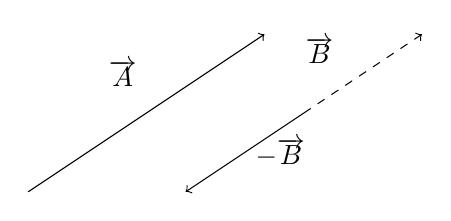
\begin{tikzpicture}
			\begin{scope}
			\coordinate (O) at (0,0);
			\coordinate (A) at (3,2);
			\coordinate (B) at (2,0);
			\coordinate (C) at (3.5,1);
			\coordinate (D) at (3.5,1);
			\coordinate (E) at (5,2);
			\draw [->] (O) -- (A);
			\draw [<-] (B) -- (C);
			\draw[->, dashed] (D) -- (E);
			\draw (1.2,1.5) node {$\overrightarrow{A}$};
			\draw (3.7,1.8) node {$\overrightarrow{B}$};
			\draw (3.2,.5) node {$-\overrightarrow{B}$};
			\end{scope}
			\end{tikzpicture}
			\caption{\koc វុិចទ័រពីរមានទិសដូចគ្នា និងទិសដៅផ្ទុយគ្នា}
		\end{figure}
	\end{multicols}
	\begin{multicols}{2}
		ដើម្បីសង់វុិចទ័រផ្គួប $\overrightarrow{C}$ យើងរំកិលវុិចទ័រ $\overrightarrow{B}$ ដោយរក្សាទិសរបស់វាទៅដាក់លើទិសនៃវុិចទ័រ $\overrightarrow{A}$ ដោយដាក់គល់នៃវុិចទ័រ $\overrightarrow{B}$ លើចុងស្លាបព្រួញនៃវុិចទ័រ $\overrightarrow{A}$។
		\begin{figure}[H]
			\centering
			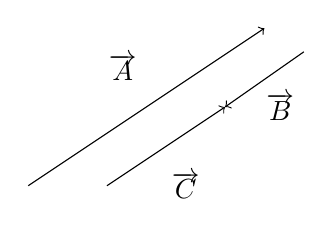
\begin{tikzpicture}
			\begin{scope}
			\coordinate (O) at (0,0);
			\coordinate (A) at (3,2);
			\coordinate (B) at (1,0);
			\coordinate (C) at (2.5,1);
			\coordinate (D) at (2.5,1);
			\coordinate (E) at (3.5,1.7);
			\draw [->] (O) -- (A);
			\draw [->] (B) -- (C);
			\draw[<-] (D) -- (E);
			\draw (1.2,1.5) node {$\overrightarrow{A}$};
			\draw (3.2,1) node {$\overrightarrow{B}$};
			\draw (2,0) node {$\overrightarrow{C}$};
			\end{scope}
			\end{tikzpicture}
			\caption{\koc ផលបូកវុិចទ័រពីរមានទិសដូចគ្នា និងទិសដៅផ្ទុយគ្នា}
		\end{figure}
	\end{multicols}	
	\begin{remark}
		ទិសដៅនៃវុិចទ័រផ្គួបគឺដូចនឹងទិសដៅនៃវុិចទ័រដែលមានអាំងតង់សុីតេធំជាងគេ។
	\end{remark}
	\item \emph{\kml ផលបូកវុិចទ័រពីរមានទិសបង្កើតបានមុំ $\theta$}
		\begin{multicols}{2}
			\quad គេមានវុិចទ័រពីរ $\overrightarrow{A}$ និង $\overrightarrow{B}$ ដែលផ្គុំគ្នាបានមុំ $\theta$ ដូចរូបខាងស្តាំ។ យើងបានវុិចទ័រផ្គួបនៃវុិចទ័រ $\overrightarrow{A}$ និង $\overrightarrow{B}$ គឺតាងដោយ $\overrightarrow{C}=\overrightarrow{A}+\overrightarrow{B}$
			\begin{figure}[H]
				\centering
				\begin{tikzpicture}
				\begin{scope}
				\coordinate (O) at (0,0);
				\coordinate (A) at (2,2);
				\coordinate (B) at (2,0);
				\coordinate (C) at (4,2);
				\draw [->] (O) -- (A);
				\draw [->] (O) -- (B);
				\draw [->] (O) -- (C);
				\draw [dashed] (2,2) --(4,2) -- (2,0);
				\coordinate[label=above:$\overrightarrow{A}$] (A) at (A);
				\coordinate[label=below:$\overrightarrow{B}$] (B) at (B);
				\coordinate[label=above:$\overrightarrow{C}$] (C) at (C);
				\pic [draw, -, "$\theta$", angle eccentricity=1.5] {angle = B--O--A};
				\end{scope}
				\end{tikzpicture}
				\caption{\koc ផលបូកវុិចទ័រពីរមានទិសបង្កើតបានមុំ $\theta$}
			\end{figure}
		\end{multicols}
		យើងអាចលើកអង្គទាំងពីរនៃសមីការនេះជាការេ
		\begin{align*}
		\text{យើងបាន}\quad :&\quad \overrightarrow{C^{2}} =\left(\overrightarrow{A}+\overrightarrow{B}\right)^{2}=\overrightarrow{A^{2}} + 2\overrightarrow{A}\overrightarrow{B}+\overrightarrow{B^{2}}=\overrightarrow{A^{2}} + 2AB\cos\left(\overrightarrow{A},\overrightarrow{B}\right) +\overrightarrow{B^{2}}\\
		\text{ដោយ}\quad :&\quad \overrightarrow{C^{2}}=C^{2},~\overrightarrow{A^{2}}=A^{2},~\overrightarrow{B^{2}}=B^{2},~\left(\overrightarrow{A},\overrightarrow{B}\right)=\theta\\
		\text{យើងបាន}\quad :&\quad C^{2}=A^{2}+B^{2} + 2AB\cos\theta\\
		\text{នាំឲ្យ}\quad :&\quad C=\sqrt{A^{2}+B^{2}+2AB\cos\theta}
		\end{align*}
	\begin{remark}
		ដើម្បីសង់វុិចទ័រផ្គួប $\overrightarrow{C}$ ដែល $\overrightarrow{C}=\overrightarrow{A}+\overrightarrow{B}$ យើងត្រូវអនុវត្តតាមវិធានអង្តត់ទ្រូងប្រលេឡូក្រាម។
	\end{remark}
	\item \emph{\kml ផលបូកវុិចទ័រពីរមានទិស និងទិសដៅកែងគ្នា}
	\begin{multicols}{2}
		\quad គេមានវុិចទ័រពីរ $\overrightarrow{A}$ និង $\overrightarrow{B}$ ដែលផ្គុំគ្នាបានមុំ $90^\circ$ ឬមានទិស និងទិសដៅកែងគ្នា ដូចរូបខាងស្តាំ។ យើងបានវុិចទ័រផ្គួបនៃវុិចទ័រ $\overrightarrow{A}$ និង $\overrightarrow{B}$ គឺតាងដោយ $\overrightarrow{C}=\overrightarrow{A}+\overrightarrow{B}$
		\begin{figure}[H]
			\centering
			\begin{tikzpicture}
			\begin{scope}
			\coordinate (O) at (0,0);
			\coordinate (A) at (2,0);
			\coordinate (B) at (0,2);
			\coordinate (C) at (2,2);
			\draw [->] (O) -- (A);
			\draw [->] (O) -- (B);
			\draw [->] (O) -- (C);
			\draw [dashed] (0,2) --(2,2) -- (2,0);
			\coordinate[label=below:$\overrightarrow{A}$] (A) at (A);
			\coordinate[label=left:$\overrightarrow{B}$] (B) at (B);
			\coordinate[label=above:$\overrightarrow{C}$] (C) at (C);
			\pic [draw, -, "$\alpha$", angle eccentricity=1.5] {angle = A--O--C};
			\end{scope}
			\end{tikzpicture}
			\caption{\koc ផលបូកវុិចទ័រពីរមានទិស និងទិសដៅកែងគ្នា}
		\end{figure}
	\end{multicols}
	យើងអាចលើកអង្គទាំងពីរនៃសមីការនេះជាការេ
	\begin{align*}
		\text{យើងបាន}\quad :&\quad \overrightarrow{C^{2}} =\left(\overrightarrow{A}+\overrightarrow{B}\right)^{2}=\overrightarrow{A^{2}} + 2\overrightarrow{A}\overrightarrow{B}+\overrightarrow{B^{2}}=\overrightarrow{A^{2}} + 2AB\cos\left(\overrightarrow{A},\overrightarrow{B}\right) +\overrightarrow{B^{2}}\\
		\text{ដោយ}\quad :&\quad \overrightarrow{C^{2}}=C^{2},~\overrightarrow{A^{2}}=A^{2},~\overrightarrow{B^{2}}=B^{2},~\left(\overrightarrow{A},\overrightarrow{B}\right)=90^\circ\\
		\text{យើងបាន}\quad :&\quad C^{2}=A^{2}+B^{2}\\
		\text{នាំឲ្យ}\quad :&\quad C=\sqrt{A^{2}+B^{2}}
	\end{align*}
\end{enumerate}
\section{ទំហំស្កាលែ}
\begin{definition}
	\emph{\kml ទំហំស្កាលែៈ} ជាទំហំដែលសំដែងដោយចំនួនពីជគណិត មិនគិតពី ទិស ទិសដៅឡើយ។ នៅក្នុងរូបវិទ្យាទំហំដែលមិនទាក់ទងនឹងទិសដៅ(ទំហំស្កាលែ) មានដូចជាៈ សីតុណ្ហភាព សម្ពាធ ថាមពល កម្មន្ត ម៉ាស រយៈពេល។ ល។\\
	\emph{\kml ឧទាហរណ៍ៈ} កីឡាករម្នាក់រត់បានចម្ងាយ $100m$ ដោយប្រើរយៈពេល $10s$។\\ ចម្ងាយ $100m$ និងរយៈពេល $10s$ ជាទំហំស្កាលែ។
\end{definition}
\section{កូអរដោនេនៃវិុចទ័រ}
	\begin{multicols}{2}
		ឧបមាថាយើងមានត្រីកោណកែង $ABC$ ដូចបង្ហាញក្នុងរូបខាងស្តាំ ។
		\begin{equation*}
			\sin\theta=\frac{\text{ជ្រុងឈម}}{\text{អុីប៉ូតេនុស}},\quad \cos\theta=\frac{\text{ជ្រុងជាប់}}{\text{អុីប៉ូតេនុស}},\quad \tan\theta=\frac{\text{ជ្រុងឈម}}{\text{ជ្រុងជាប់}}
		\end{equation*}
		\begin{figure}[H]
			\centering
			\begin{tikzpicture}
				\centering 
				\begin{scope}
				\large
				\coordinate (C) at (0,0);
				\coordinate (A) at (3,0);
				\coordinate (B) at (3,2);
				\draw (C) -- (A) -- (B) -- cycle;
				\pic [draw, -, "$\theta$", angle eccentricity=1.5] {angle = A--C--B};
				\draw (A) -- ++ (0, .3cm) -- ++ (-.3cm, 0) -- ++ (0, -.3cm);
				\coordinate[label=below:$A$] (A) at (A);
				\coordinate[label=above:$B$] (B) at (B);
				\coordinate[label=below:$C$] (C) at (C);
				\coordinate[label=below:{\text{ជ្រុងជាប់}}] (1.5,0) at (1.5,0);
				\coordinate[label=right:{\text{ជ្រុងឈម}}] (3,1) at (3,1);
				\coordinate[label=right:{\text{អុីប៉ូតេនុស}}] (-1,1) at (-1,1);
				\end{scope}
			\end{tikzpicture}
			\caption{\koc ទំនាក់ទំនងក្នុងត្រីកោណមាត្រ}
		\end{figure}
	\end{multicols}
	ទំនាក់ទំនង់រវាង $\sin\theta$ និង $\cos\theta$ គឺ
	\begin{align*}
		\tan\theta=\frac{\sin\theta}{\cos\theta} \quad \text{និង}\quad \sin^{2}\theta+\cos^{2}\theta=1
	\end{align*}
	\begin{multicols}{2}
		គេមានវុិចទ័រ $\overrightarrow{A}$ ស្តិតក្នុងប្លង់ $xy$ និងបង្កើតបានមុំ $\theta$ ជាមួយអ័ក្ស $Ox$ ដូចរូប។\\ យើងចំណោលកែងវុិចទ័រ $\overrightarrow{A}$ លើអ័ក្ស $Ox$ និង $Oy$ យើងបានធាតុរបស់វា{\en(Components of Vectors)}គឺ $\overrightarrow{A_{x}}$ និង $\overrightarrow{A_{y}}$។ តាមលក្ខណៈនៃវុិចទ័រយើងបានៈ $\overrightarrow{A}=\overrightarrow{A_{x}}+\overrightarrow{A_{y}}$
		\begin{figure}[H]
			\centering
			\begin{tikzpicture}
			\begin{scope}
			\coordinate (O) at (0,0);
			\coordinate (x) at (3,0);
			\coordinate (y) at (0,3);
			\coordinate (A) at (2,2);
			\draw [->] (O) -- (x);
			\draw [->] (O) -- (y);
			\draw [->] (O) -- (A);
			\draw [dashed] (0,2) --(2,2) -- (2,0);
			\coordinate[label=below:$x$] (x) at (x);
			\coordinate[label=left:$y$] (y) at (y);
			\coordinate[label=above:$\overrightarrow{A}$] (A) at (A);
			\coordinate[label=below:$\overrightarrow{A_{x}}$] (2,0) at (2,0);
			\coordinate[label=left:$\overrightarrow{A_{y}}$] (0,2) at (0,2);
			\coordinate[label=below:$O$] (0,0) at (0,0);
			\pic [draw, -, "$\theta$", angle eccentricity=1.5] {angle = x--O--A};
			\end{scope}
			\end{tikzpicture}
			\caption{\koc ផលបូកវុិចទ័រពីរមានទិស និងទិសដៅកែងគ្នា}
		\end{figure}
	\end{multicols}
	\begin{proof}
		\begin{align*}
			\text{ដែល}\quad :&\quad A_{x}=A\cos\theta \quad\text{និង}\quad A_{y}=A\sin\theta\\
				\text{យើងបាន}\quad :&\quad \overrightarrow{A^{2}} =\left(\overrightarrow{A_{x}}+\overrightarrow{A_{y}}\right)^{2}=\overrightarrow{A^{2}_{x}} + 2\overrightarrow{A_{x}}\overrightarrow{A_{y}}+\overrightarrow{A_{y}^{2}}=\overrightarrow{A៌_{x}^{2}} + 2A_{x}A_{y}\cos\left(\overrightarrow{A_{x}},\overrightarrow{A_{y}}\right) +\overrightarrow{A_{y}^{2}}\\
			\text{ដោយ}\quad :&\quad \overrightarrow{A^{2}}=A^{2},~\overrightarrow{A_{x}^{2}}=A_{x}^{2},~\overrightarrow{A_{y}^{2}}=A_{y}^{2},~\left(\overrightarrow{A_{x}},\overrightarrow{A_{y}}\right)=90^\circ\\
			\text{យើងបាន}\quad :&\quad A^{2}=A_{x}^{2}+A_{y}^{2}\\
			\text{នាំឲ្យ}\quad :&\quad A=\sqrt{A_{x}^{2}+A_{y}^{2}}
		\end{align*}
	\end{proof}